\chapter{Implementation}

The system designed for this research contains four major pieces: A Partitioning
application, A Visualization tool, The Rendering Component, and the Selection
Algorithm. Below is a detailed explanation of their implementation and theory.

\section{Partitioning Application}

The partitioning application is a standalone command line application that reads
from a number of binary point data files. It creates the different partitioning
systems needed to evaluate the algorithm implementations and stores them in a
custom binary format for ease of access at runtime. The files have been designed
so that they can be accessed via the local file system or through a web server.

The data structure has been partitioned such that each level in the tree
structure, for both the Octree and Icosatree, contains points which are left in
each node. The nodes are split into a sub-cell grid structure so all nodes at a
specific depth are uniformly dense in order for the level of detail algorithm to
only have to deal with screen area and not point densities within the
visualization tool when determining how deep to traverse. The data also contains
information defining the number of points in the node, the number of child
nodes, and the layout of the binary data (at the root, only).

The structure of the Octree and Icosatree file systems are fairly
straightforward. Each is defined by a file tree originating at a given root
directory. Then in each directory, including the root, a point data file exists
along with an ASCII text file containing a list of the existing child nodes at
that location. The root directory also contains a CSV file defining the binary
layout of the point data which contains information about attributes: name,
offset, data type, size in bytes, min, max, mean, and variance.

The Octree and Icosatree structures are identical except for the fact that each
Octree cell contains, at most, eight child cells. The Icosatree root node can
contain up to twenty child cells and each cell after that can contain at most
eight. The Octree structure is split along the XYZ axes as in Figure 2. However,
the Icosatree is split into twenty triangular prism cells at the root as in
Figure 5. Below that, each cell is split into eight additional triangular prisms
as seen in Figure 6 and Figure 7.

\begin{figure}[htp]
\begin{center}
  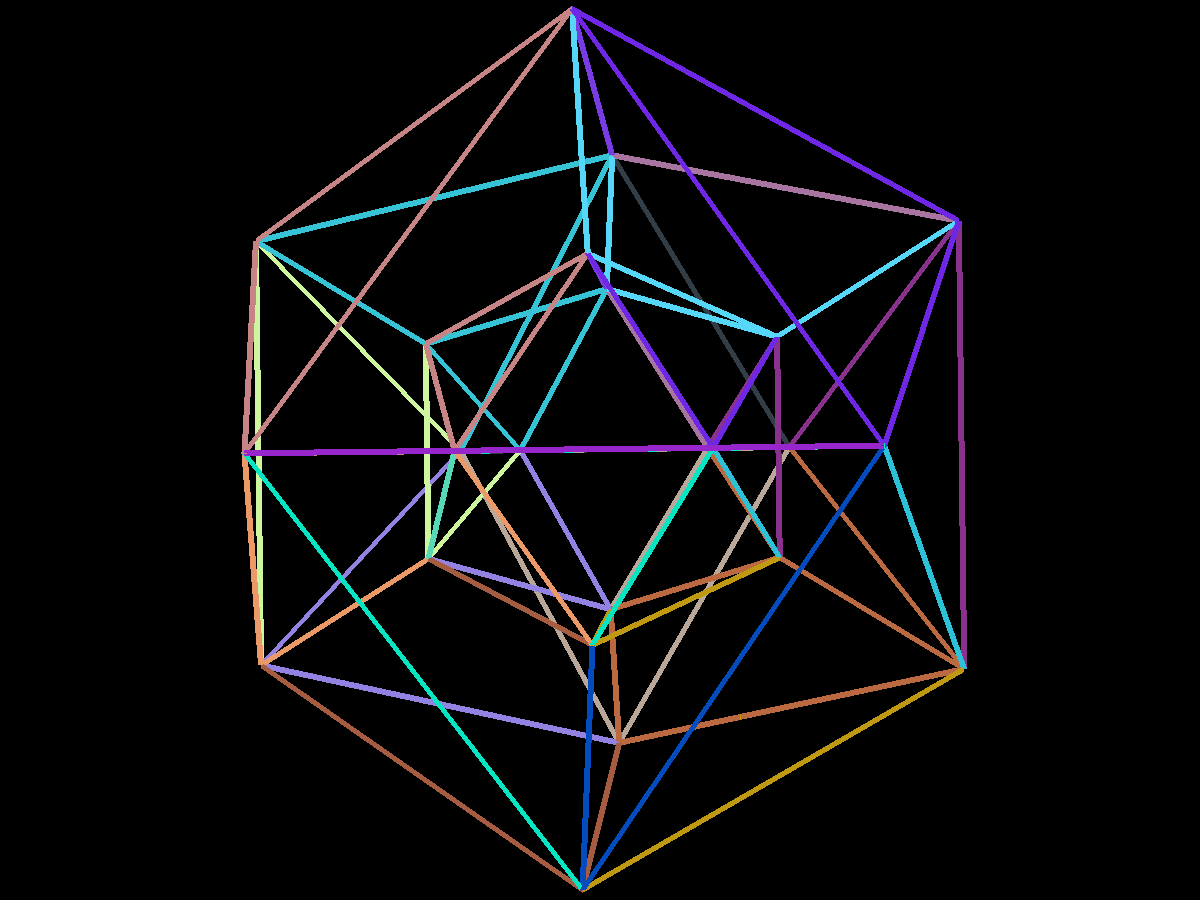
\includegraphics[width=.75\linewidth]{images/trianglePrismBounds.png}
  \caption{Icosatree Wireframe}
  \label{fig:tpv}
\end{center}
\end{figure}

\begin{figure}[htp]
\begin{center}
  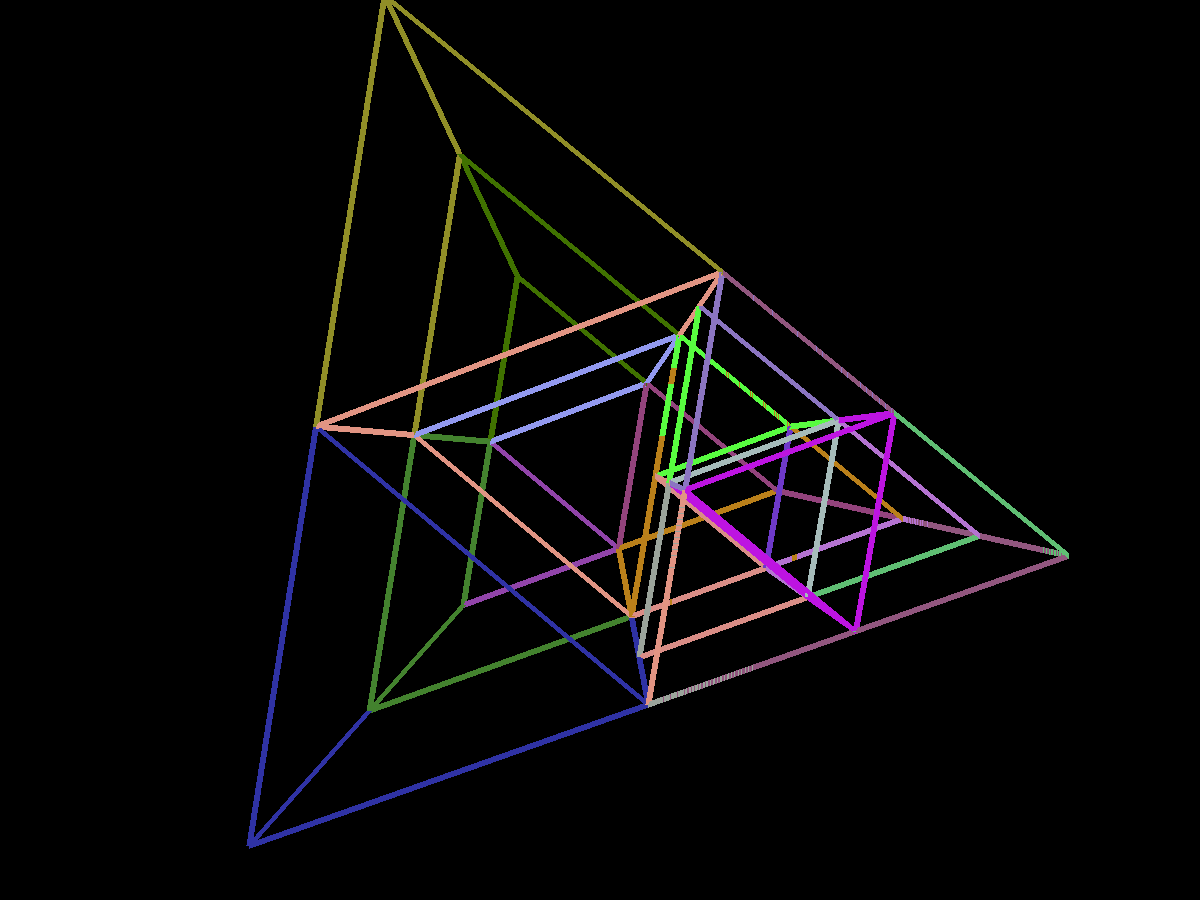
\includegraphics[width=.75\linewidth]{images/trianglePrismBoundsSplit.png}
  \caption{Triangle Prism Partitioning}
  \label{fig:tpvSplit}
\end{center}
\end{figure}

\begin{figure}[htp]
\begin{center}
  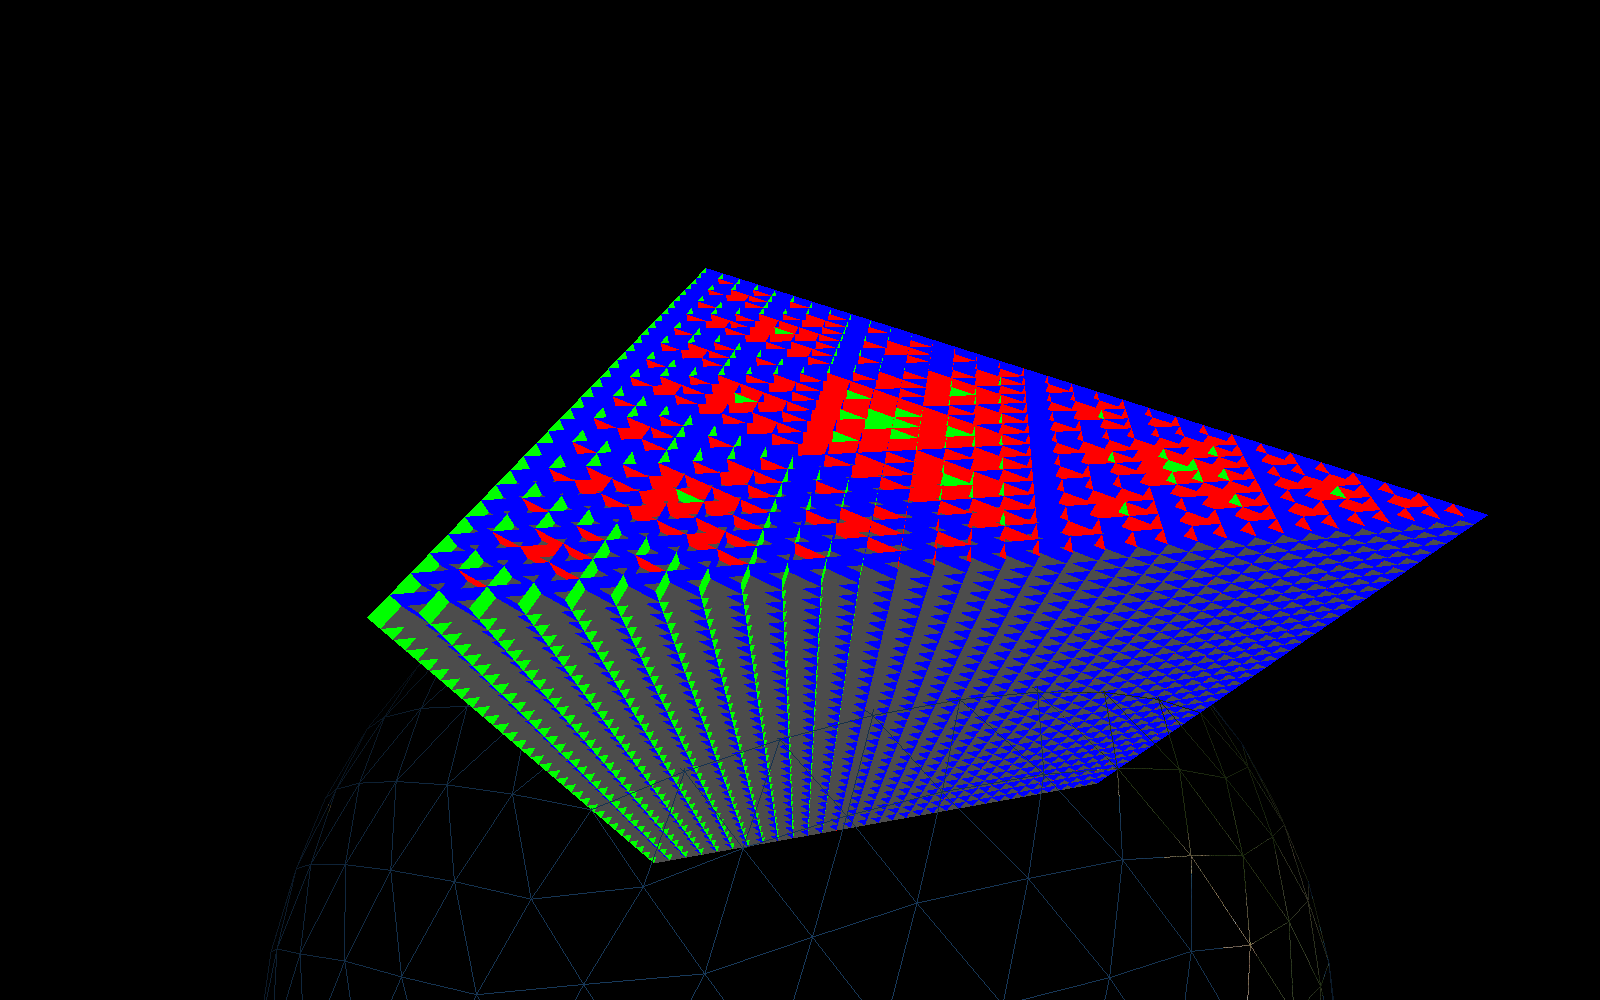
\includegraphics[width=.9\linewidth]{images/treeStructure_depth5.png}
  \caption{Icosatree Cells - Depth 5}
  \label{fig:icosatreeCells}
\end{center}
\end{figure}

Each cell is also split into sub-cells; this allows the tree creation to
guarantee uniform density of point data at any specific level of the tree which
greatly simplifies level of detail calculations in the renderer. As the tree
structure is built, a point is inserted into the root node. The sub-cell is
computed and if no point was previously added there, the current point is
stored. If a point was previously stored at that sub-cell index, the point
closest to its centroid is left there and the remaining point is sent to one of
the cells' child cells. This continues until all points have been added to the
tree. Once that is complete, the command line tool writes the tree structure as
a set of directories and binary or ASCII files. A subset of this file structure
can be seen in \ref{fig:fileStructure}. The DAT file contains the binary point data and the
text file contains the child cell index values which contain point data of their
own. These child cells also have a sub-directory within that nodes’ directory
which continues to the leaves of the tree.

\begin{figure}[htp]
\begin{center}
  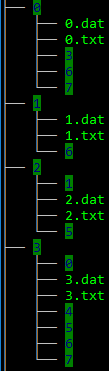
\includegraphics[height=3.0in]{images/filestructure.png}
  \caption{Tree File Structure}
  \label{fig:fileStructure}
\end{center}
\end{figure}

\section{Visualization Tool}

The visualization tool consists of a Java/OpenGL rendering system based off the
Java OpenGL Library (JOGL) and a rendering toolkit the author has developed.
Simple geospatial navigation and terrestrial terrain have been added as they aid
the user when interacting and visualizing this form of data. The visualization
renders a simple WGS84 projected globe, a spherical orbit navigator, the point
cloud renderer which supports the different data structures implemented by the
partitioning application, and the selection algorithm used by the user which
allows them to select objects, as the points that comprise them, from the scene
using a screen-space lasso tool.

The visualization tool renders each item in the scene as its own scene element.
The camera navigation is based on a geospatial anchor point and an
azimuth/elevation/distance offset from the anchor. A local origin will offset
the scene component's local coordinate system for floating point precision
reasons and each scene element will update its own position based on this local
origin.

There was also the need for a renderable Earth scene element \ref{fig:earth}.
This was developed by creating a GeodesicCoordinate to base the geometry from. The first level of
detail consists of a number of rectangular sections each thirty degrees on a
side. Then, as the camera moves closer to the surface, each portion splits into
smaller sections \ref{fig:earthWire}. In order to display accurate elevation
data, support for Digital Elevation Model data was added and used as a lookup
dataset for elevation values at each vertex \ref{fig:earthDEM}. Initially, a
single high resolution texture was used for the imagery but even an 8k image did
not add enough fidelity as the user zoomed close enough into the terrain so
support was also added for the Slippy Map Tile URL protocol; specifically,
OpenStreetMap and Stamen Terrain imagery \ref{fig:earthTiles}. The Digital
Elevation Model data is downloadable manually and is indexed the first time the
Visualization application is run whereas the imagery is accessed via HTTP
requests as it is needed.

\begin{figure}[htp]
\begin{center}
  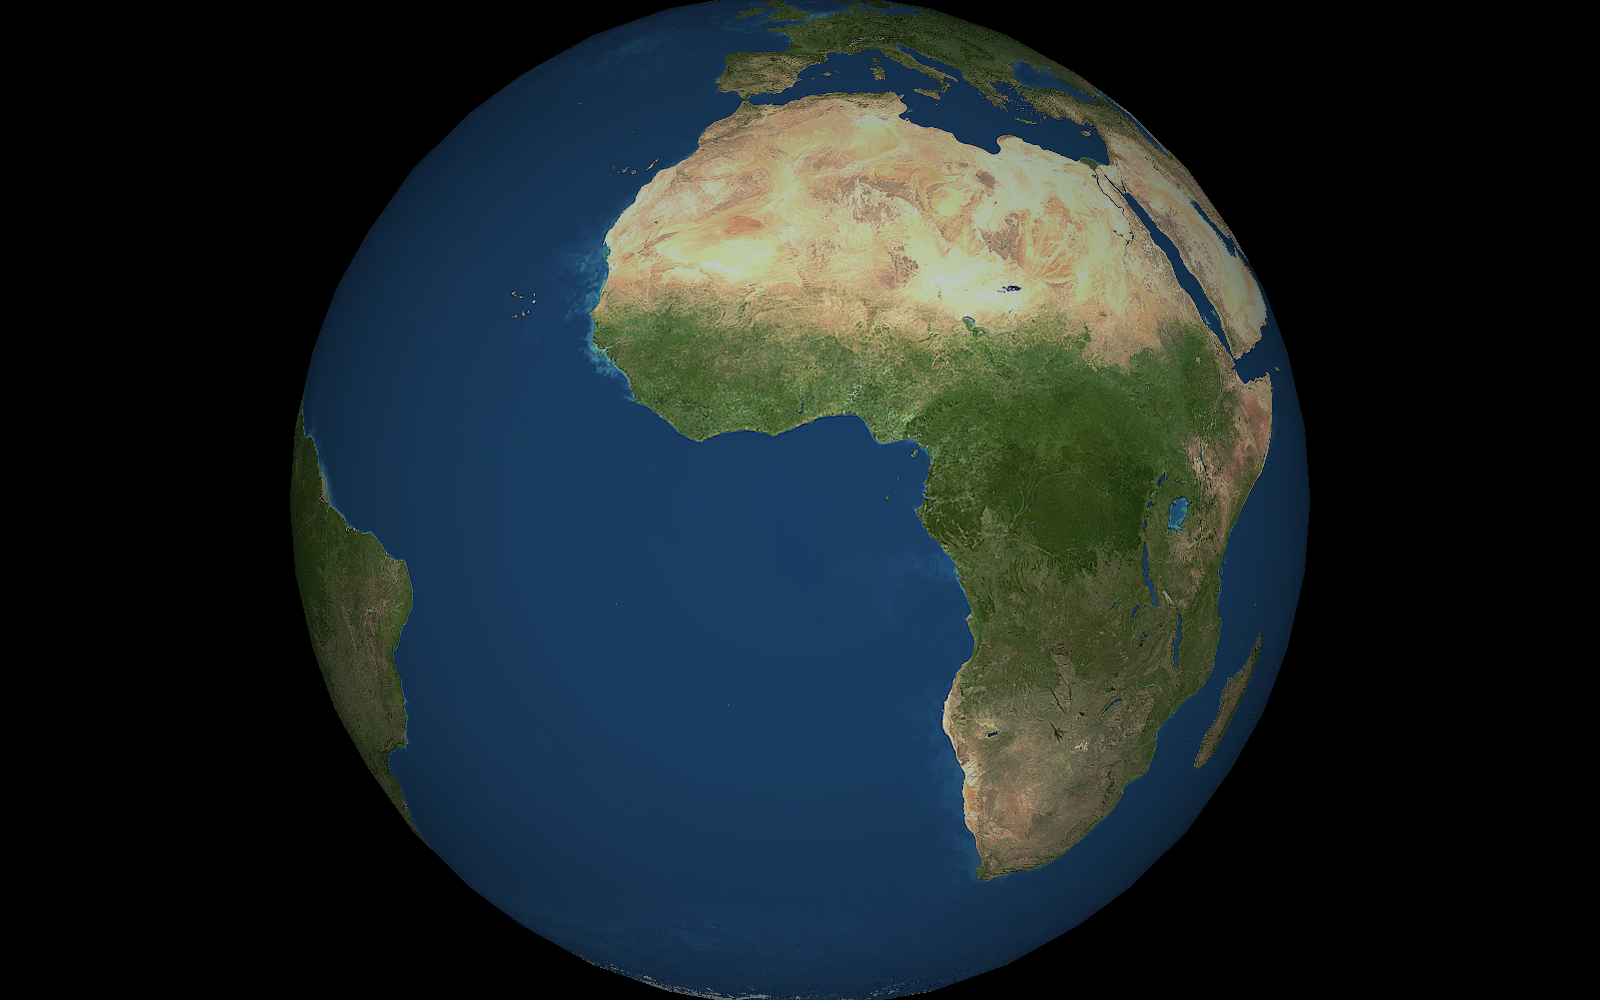
\includegraphics[width=.75\linewidth]{images/earth.png}
  \caption{Earth}
  \label{fig:earth}
\end{center}
\end{figure}

\begin{figure}[htp]
\begin{center}
  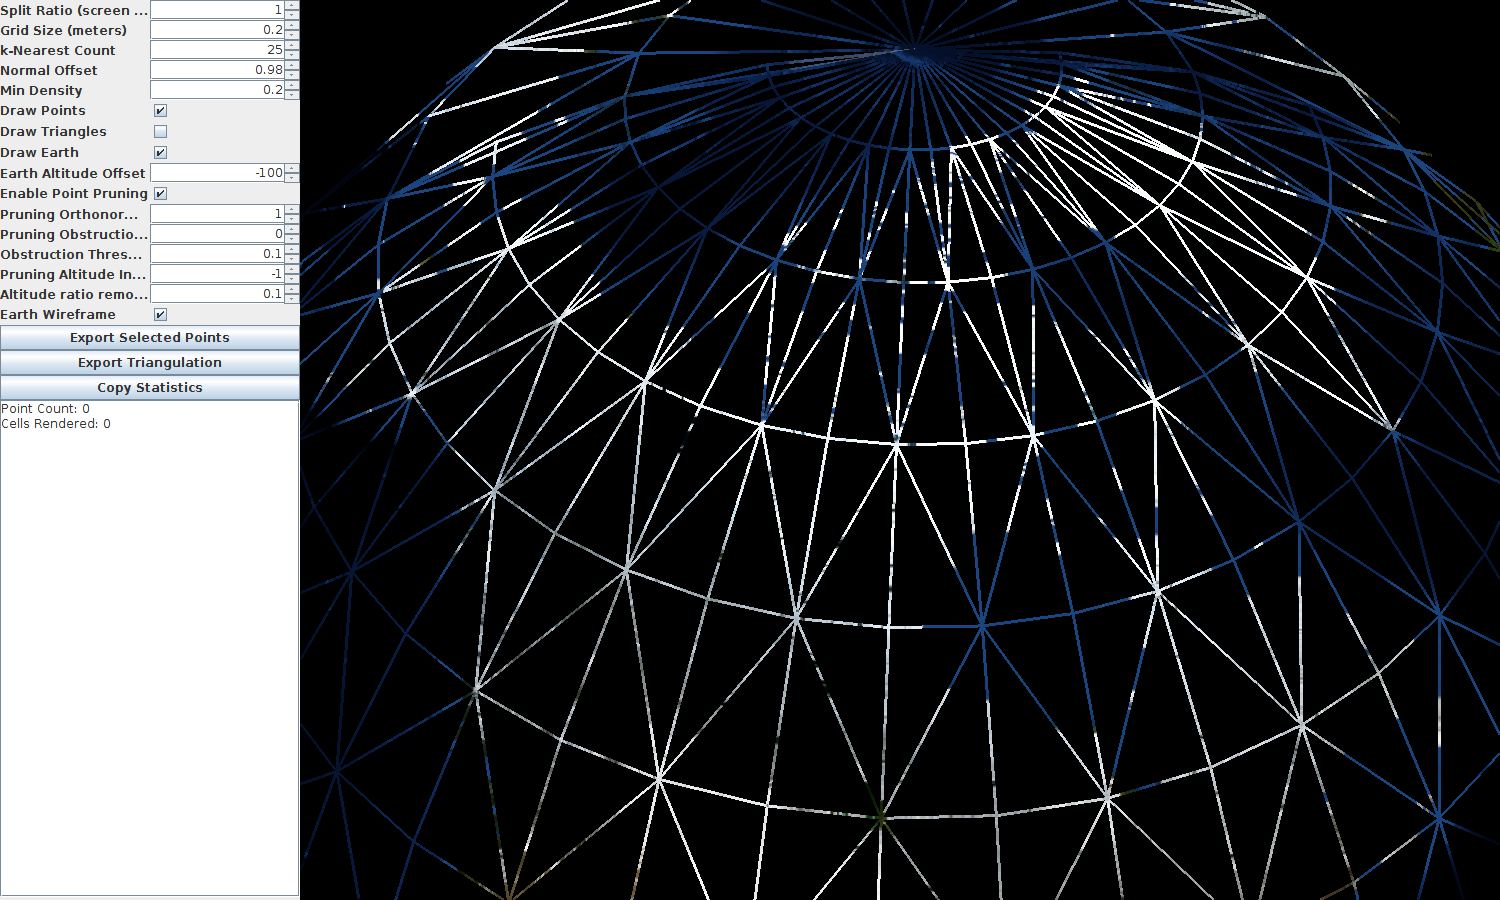
\includegraphics[width=.75\linewidth]{images/earthlod.png}
  \caption{Earth Wireframe}
  \label{fig:earthWire}
\end{center}
\end{figure}

\begin{figure}[htp]
\begin{center}
  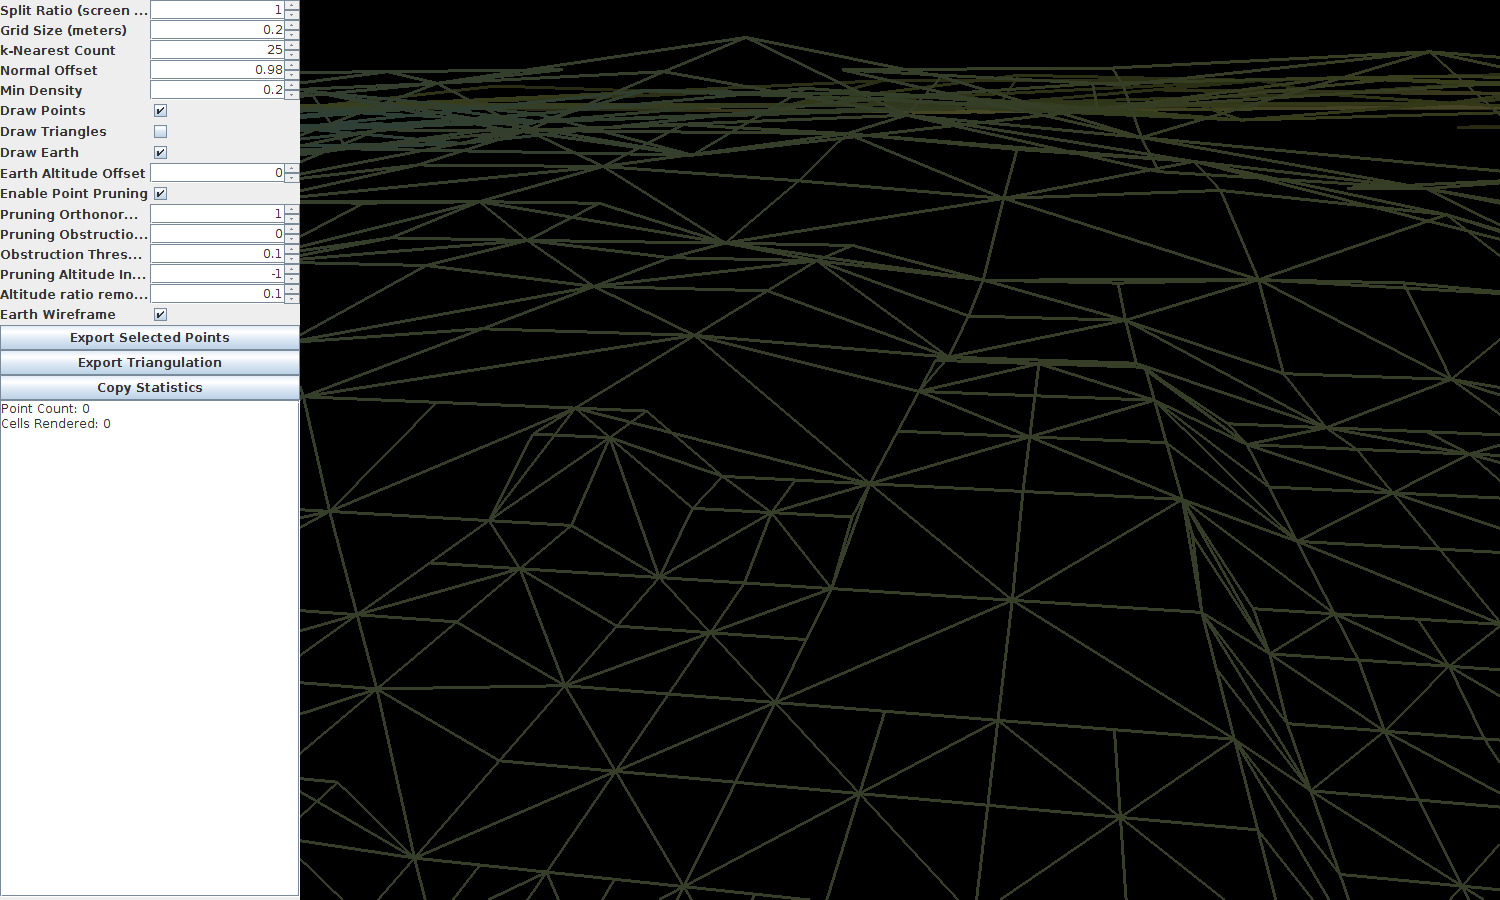
\includegraphics[width=.75\linewidth]{images/earthElevation.png}
  \caption{Earth Elevation}
  \label{fig:earthDEM}
\end{center}
\end{figure}

\begin{figure}[htp]
\begin{center}
  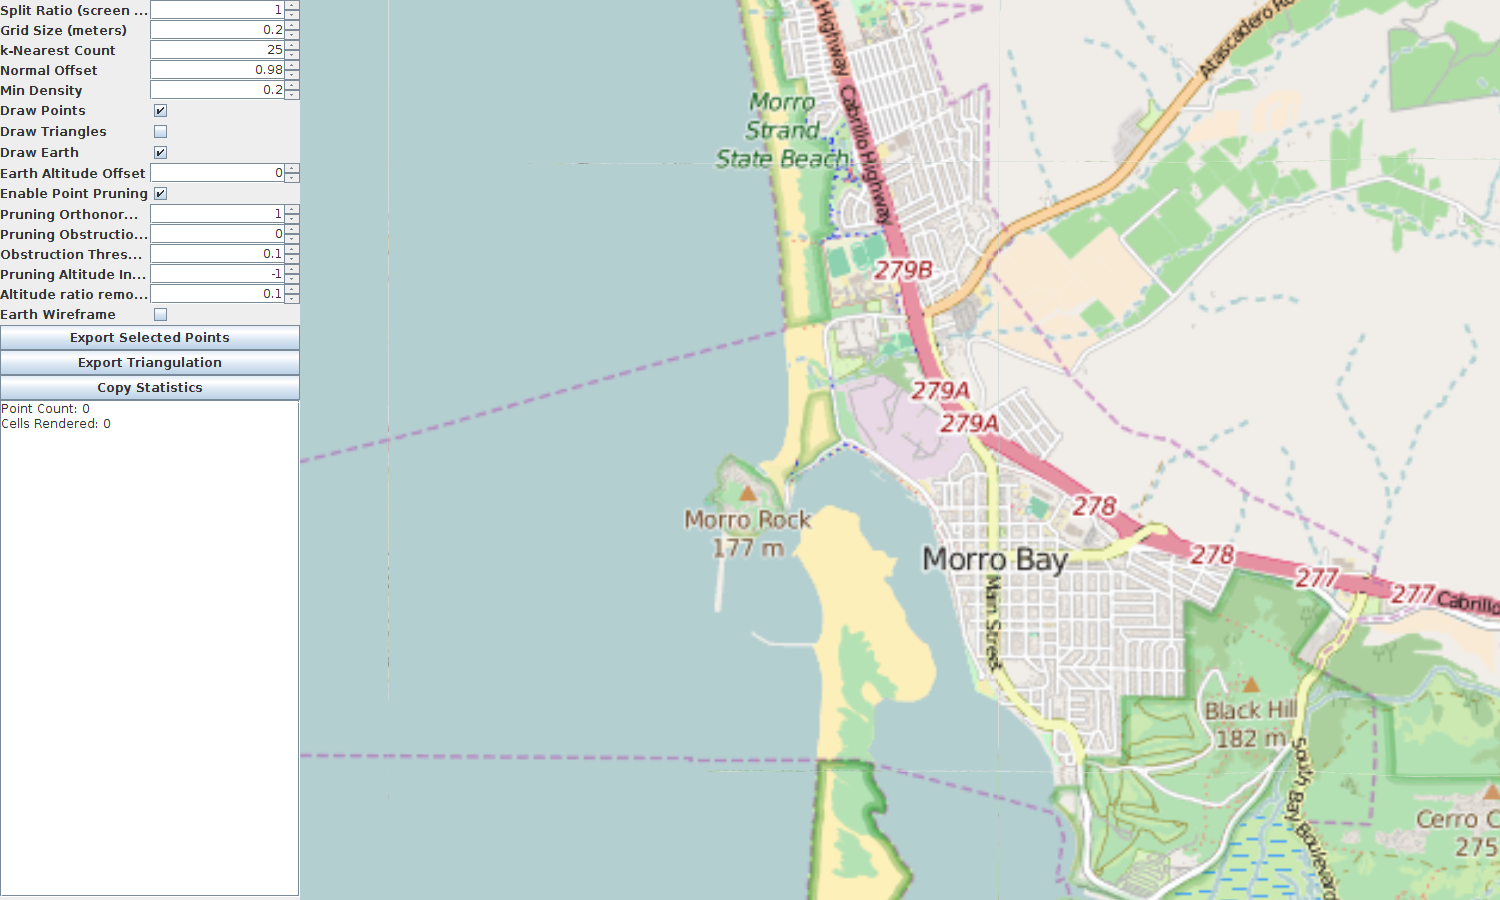
\includegraphics[width=.75\linewidth]{images/earthTiles.png}
  \caption{OpenStreetMap Tiles}
  \label{fig:earthTiles}
\end{center}
\end{figure}

\section{Rendering Component}

The rendering component initially reads the root node and attributes layout
information from the dataset (locally or over the web). It then uses the
bounding volume of the node to determine if it should be rendered or not and if
its children should be queried. It then uses a screen-space level of detail
algorithm to determine how deep to traverse; this depth will be tunable based on
user preference.

The Octree and Icosatree are both supported by the rendering component as their
data structures are identical aside from the number of children their root nodes
may contain. The class TreeRenderable is given a path (either local or HTTP) to
the root of the tree data and a ConnectionType.  Each frame, it does a frustum
culling pass to determine which tree cells should be included in the rendering
step. Then, for each cell it checks its on-screen area. This area calculation is
used to compare against two different thresholds; the first is if this node
should render any points it may contain (50×50 pixels) and the second is if its
children should be checked (200×200 pixels). The nodes are split into two sets;
those that are complete and those that are pending. The complete nodes have
their point data already retrieved while the pending nodes have been created but
are still waiting for their point data to be accessed by the connection thread.
Next, a small portion of the frame time is given over for uploading data to the
graphics card; this is limited in order to keep the visualization at an
interactive frame rate. The vertex buffer implementation is actually a number of
buffer pools, each of which contain a number of vertex buffer objects and the
pool is able to allocate and delete these objects as needed. The tree structure
contains the maximum number of points necessary for any node in the tree; this
is the starting segment size for the buffer pools. The first pool is defined by
a number of segments (100 by default) which can each hold this maximum number of
points per buffer object (byte size equal to the attribute-stride * max points *
segments per buffer). Then, another pool is made by dividing the segment size by
two and continuing this until the smallest buffer object is sliced into segments
less than 100 points long. This allows a number of different sized cells to be
inserted into a buffer that, at least, fills half of its total capacity but also
allows the rendering system to intelligently add, remove, and update cells in
the tree without having to pack or rearrange data on the graphics card every
frame. Below, in \ref{fig:visualization}, is a screenshot of Morro Bay in California; this
is a subset of the San Simeon, CA point cloud dataset and, in total, contains
13,725,592 points. At the current zoom distance and level of detail the
rendering component is only required to render around three million points.

\begin{figure}[htp]
\begin{center}
  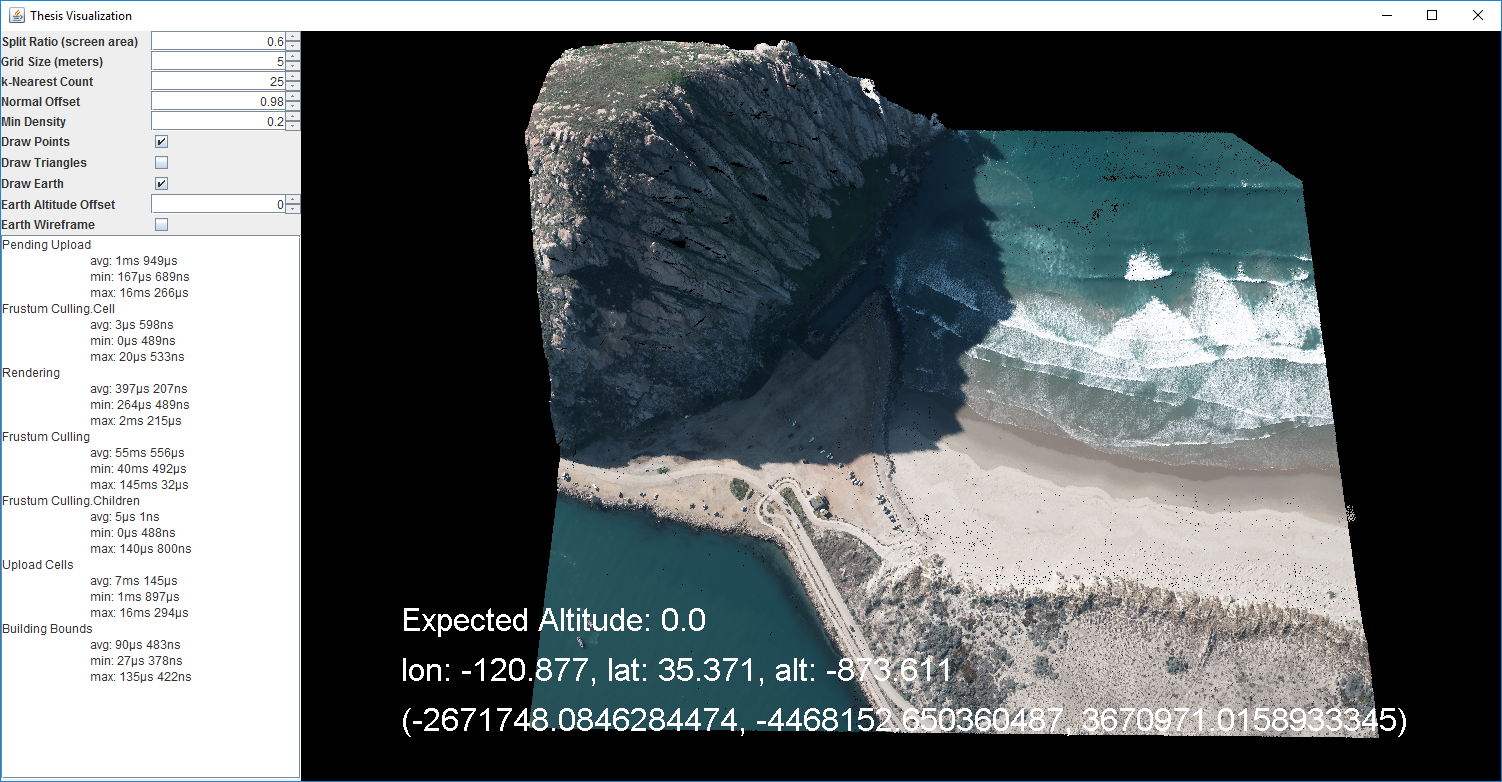
\includegraphics[width=.9\linewidth]{images/visualization.png}
  \caption{Visualization Application with Small Point Cloud}
  \label{fig:visualization}
\end{center}
\end{figure}

The TreeRenderable itself controls how the point data is
displayed in the visualization application. It creates a custom-built vertex
buffer object pool which is then used to store and render the point data. The
buffer pool contains a set of smaller pools internally that are defined by a set
segment size (number of points available in a block) and a number of available
segments. Each of these smaller pools is able to append itself with as many
vertex buffer objects as it needs and uses a global index to find the specific
segment location that is bound to each tree cell. When a segment is cleared, any
empty vertex buffer objects on a segment pool will also be removed in order to
free up memory. When the Tree Cells are uploaded to the GPU, the segment pool
with the smallest segment size that will fit the tree cell's point count will be
selected. Then, the first available index in that cell will be requested and the
tree cell will store this pool index and segment index for rendering later. The
number of internal segment pools is defined by the maximum number of points any
given tree cell will contain in the point cloud collection. \ref{fig:flowchart}
is a flow chart that goes through the steps in the rendering pass for the TreeRenderable.

\begin{figure}[htp]
\begin{center}
  \includegraphics[width=.9\linewidth]{images/TreeRenderer_flowchart.png}
  \caption{TreeRenderer Flow Chart}
  \label{fig:flowchart}
\end{center}
\end{figure}

\section{Selection Algorithm}

The selection algorithm attempts to apply portions of two separate point cloud
selection algorithms to the same set of data. The Screen-Space Operator
Algorithm \cite{1_VAST:VAST11:105-112} is used to define surfaces inside the
point cloud; this is useful for visualizing the walls of buildings and such.
However, the algorithm itself doesn't handle selection of objects. The CAST
algorithm \cite{2_yu:hal-01178051} allows selection of more dense portions of a
point cloud via two-dimensional mouse selection but it requires a dense cloud of
points to handle selection. I have attempted to apply the screen-space lasso and
point density techniques from the CAST algorithm and apply the surface creation
and triangulation algorithm to the resulting selection in order to give a user
more utility when analyzing a point cloud dataset.

The first step of the algorithm is for the user to define the search area. This
is done in the visualization by holding the control key and holding the left
mouse button while defining the lasso area. The shape is automatically connected
to the initial selection point as the user outlines the lasso shape but the
final polygon will be automatically closed the first time the lasso crosses
itself in order to create a closed loop.

Then, a simple volume frustum is created from the camera into the scene along
the screen-space lasso polygon. The tree is searched and any points that are
contained within the lasso are returned. Next, for each point, the k-nearest
neighboring points are queried and a covariance matrix is computed. If the
normal of the best-fit plane of the entire selection is parallel (or within a
user-defined threshold) the point is dropped from the selection. Finally, any
points whose most distant neighbor is further than twice the user-defined grid
size is also removed. This removes any points that are parallel to the ground as
well as any points that are in small groups and aren't useful (less than the
k-nearest limit).

In order to handle triangulation, the Screen-Space Operator Algorithm is used to
determine which points in the selection are unobstructed. This is done by
projecting a ray from each point towards the camera and, if any other point is
within a specified angular distance and closer to the camera than the tested
point, it is removed. These points are then converted into a two-dimensional
plane and a Delaunay triangulation algorithm is used to triangulate them. A map
of the 2D projected point to the original 3D point is used to convert this
triangulation back into a useful triangle mesh. The lasso (\ref{fig:lasso}),
point selection (\ref{fig:pointSelection}), and triangle mesh
(\ref{fig:triangulation}) can be seen below. The follwing is pseudocode for the
Selection Algorithm:

\begin{enumerate}
  \item User Selects Area Of Screen
  \item Create closed polygon from set of screen coordinates
  \item Create projected 3D volume from 2D polygon
  \item Get volume intersection on visible point data
  \item If Pruning enabled, prune points based on user settings
  \begin{enumerate}
    \item Apply the following in User Order
    \begin{itemize}
      \item Orthonormal Pruning
      \begin{enumerate}
        \item Compute global eigenvector for plane normal vector
        \item For-each point, compute engenvector using k-nearest neighbors
        \item if point eigenvector is within user-defined angle of global normal, discard
      \end{enumerate}
      \item Obstruction Pruning
      \begin{enumerate}
        \item For-each point, if any other point is closer to the camera and the angle between the two points is within a user-defined threshold, discard
      \end{enumerate}
      \item Altitude Pruning
      \begin{enumerate}
        \item Compute min/max altitude of all input points
        \item For-each point, if altitude is within user-defined threshold of min value, discard
      \end{enumerate}
    \end{itemize}
  \end{enumerate}
  \item If user enabled, Draw Points
  \item If user enabled, Compute Triangle Mesh
    \begin{enumerate}
      \item Project points to Screen Space
      \item Remove any occluded points
      \item Compute Mesh using Delaunay Triangulation
      \item Project triangulation to World Space
      \item Render Triangle Mesh
    \end{enumerate}
\end{enumerate}

\begin{figure}[htp]
\begin{center}
  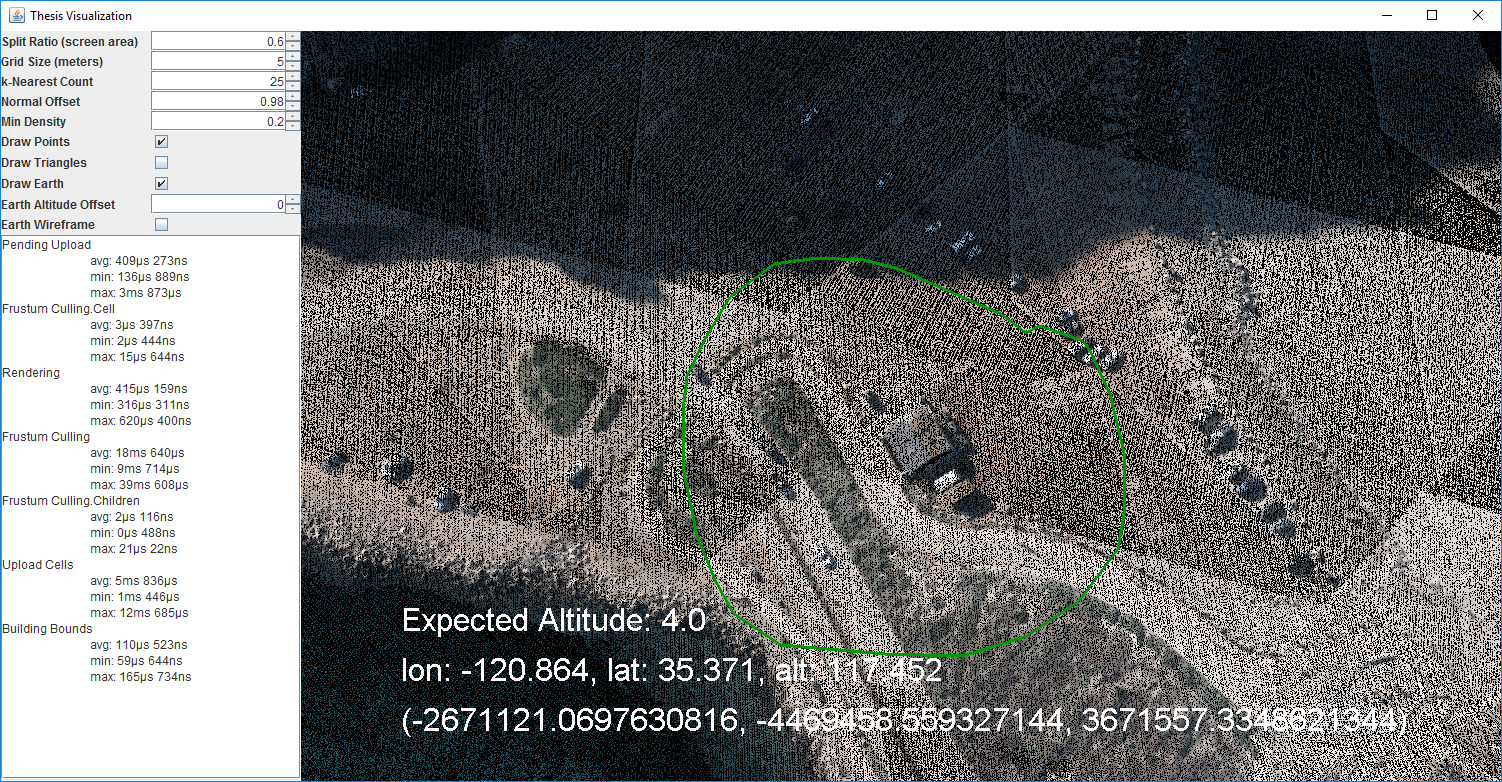
\includegraphics[width=.75\linewidth]{images/lasso.png}
  \caption{Selection Lasso}
  \label{fig:lasso}
\end{center}
\end{figure}

\begin{figure}[htp]
\begin{center}
  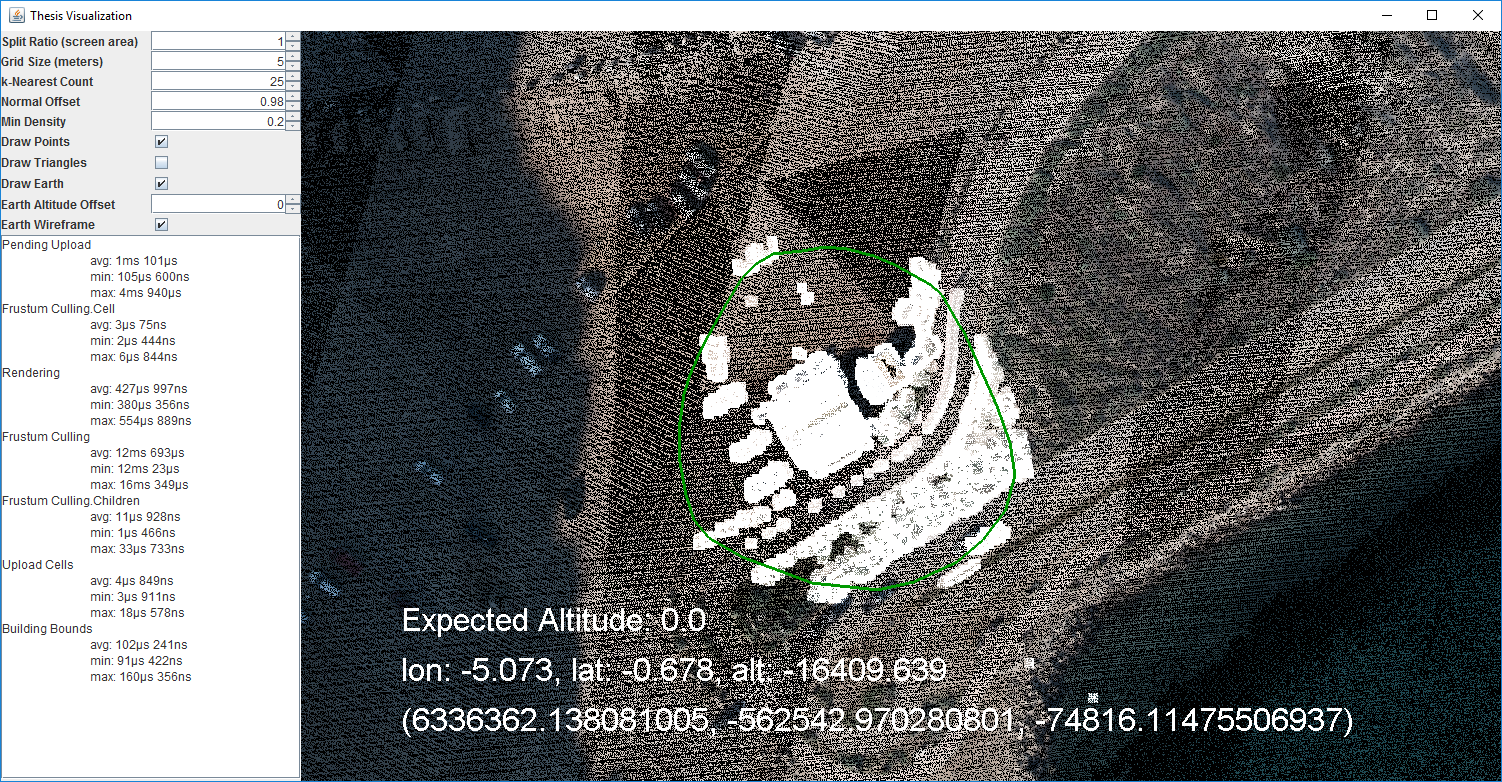
\includegraphics[width=.75\linewidth]{images/pointSelection.png}
  \caption{Point Selection}
  \label{fig:pointSelection}
\end{center}
\end{figure}

\begin{figure}[htp]
\begin{center}
  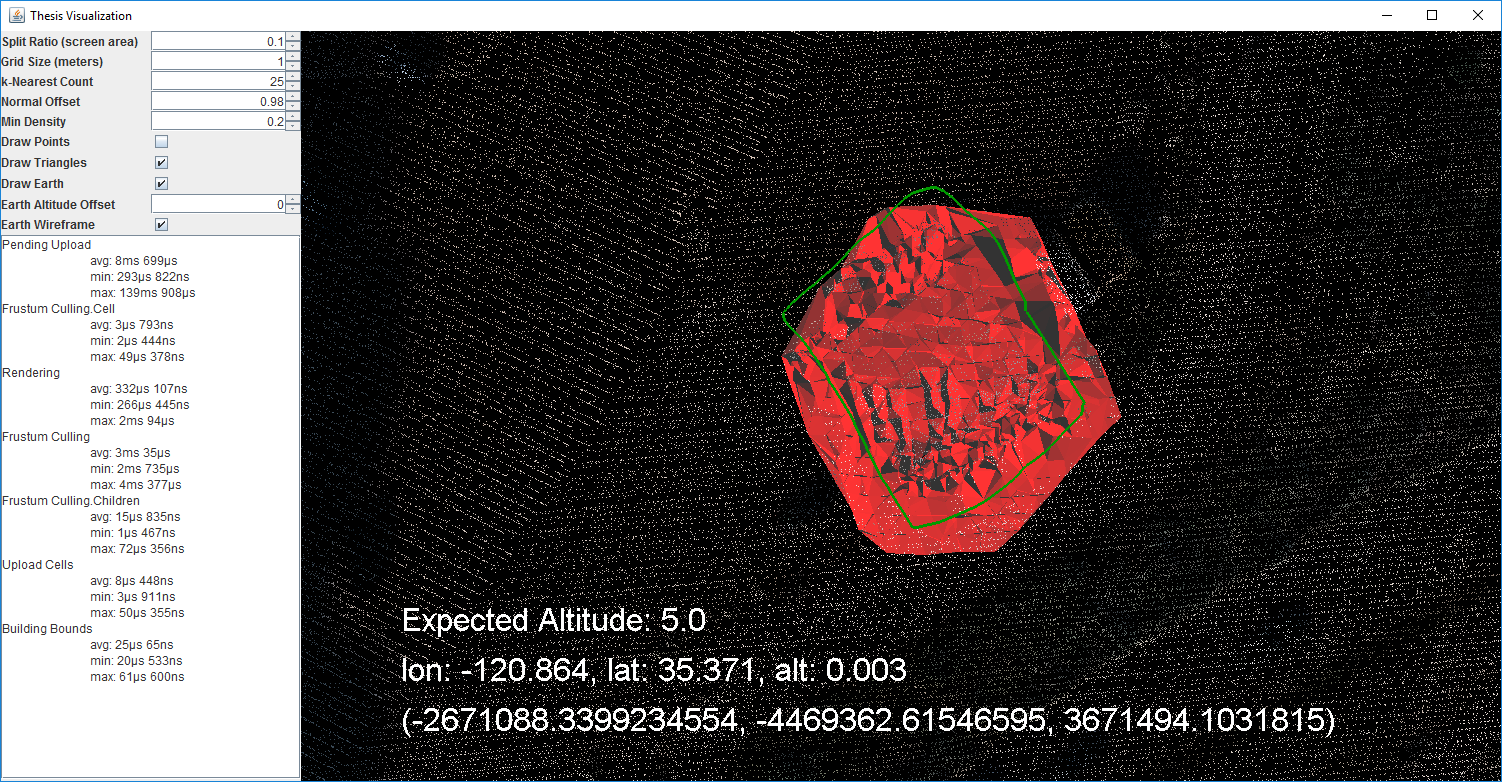
\includegraphics[width=.75\linewidth]{images/triangulation.png}
  \caption{Point Triangulation}
  \label{fig:triangulation}
\end{center}
\end{figure}
